\chapter{Data and simulation}
\label{data}

In this section, we go over data sources, perform parameter calibrations and derive all investment strategies for our simulation.

\section{Data sources}

We use historical monthly BIST 30\footnote{BIST 30 is an index measuring the stock performance of 30 largest companies in Turkey} and REIDIN\footnote{REIDIN provides residential sales price index for Turkey, using data, covering $200,000$ house listings in 62 cities and 221 counties, per month, weighted by population, and calculated using Laspeyres' formula.} data from 2004 to 2014, to construct stock and house price series respectively. Figures \ref{fig:bist30} and \ref{fig:reidin} illustrate the general upward trend in both series, with a collapse during 2008 crisis.

\begin{figure}[h!]
	\centering
    \begin{minipage}{0.45\textwidth}
		\centering
		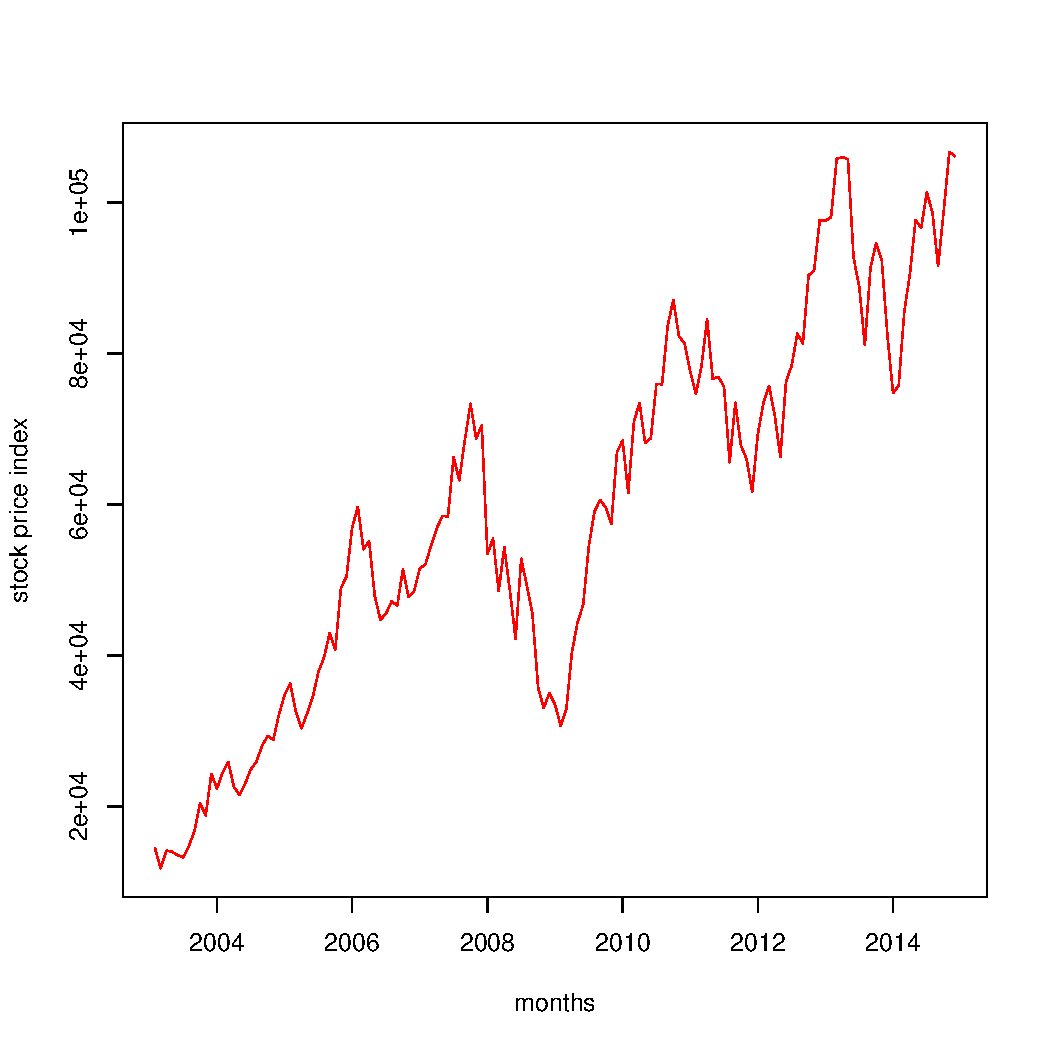
\includegraphics[scale=0.4]{figs/bist.pdf}
		\caption{BIST30 Turkish stock market prices}
		\label{fig:bist30}
	\end{minipage}
	\hfill
    \begin{minipage}{0.45\textwidth}
		\centering
		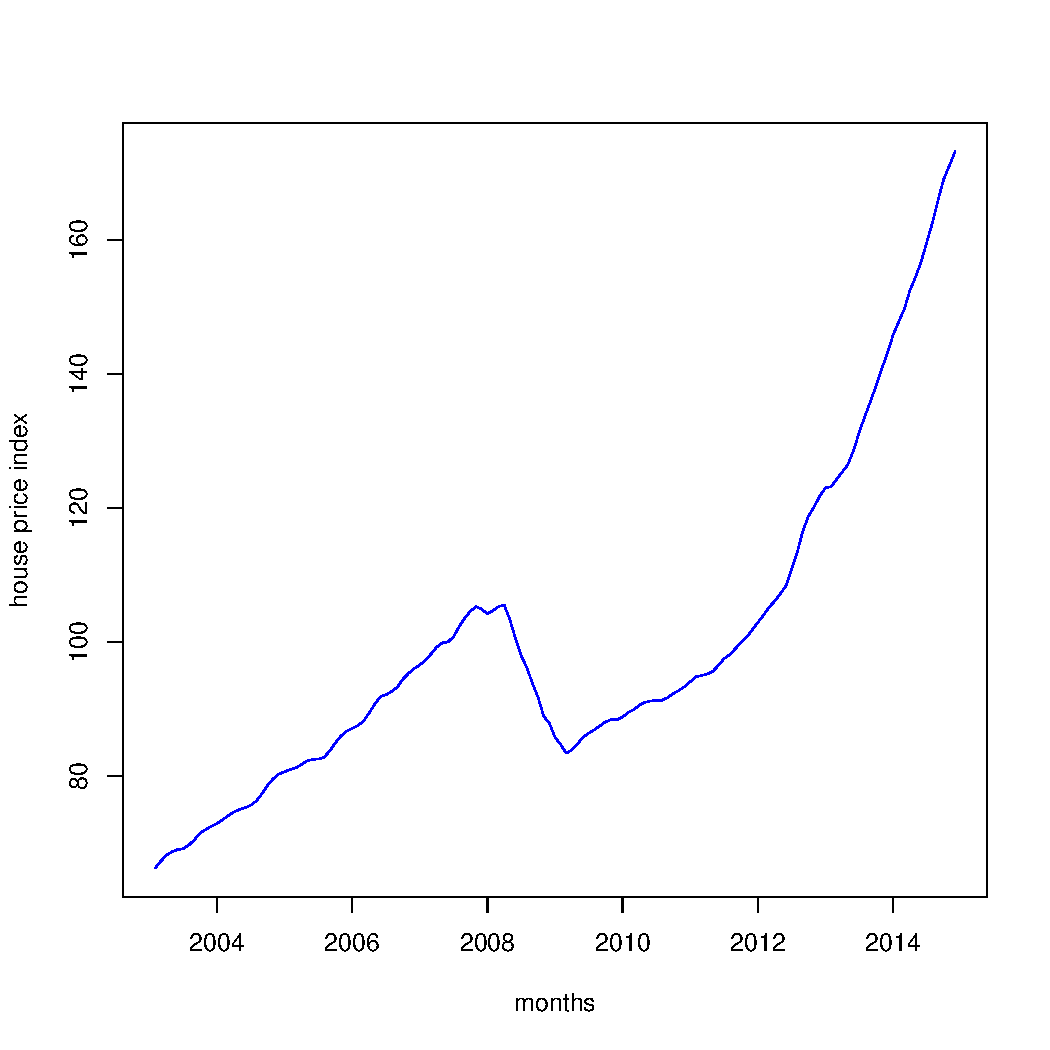
\includegraphics[scale=0.4]{figs/reidin.pdf}
		\caption{Reidin Turkish house price index}
		\label{fig:reidin}
	\end{minipage}
\end{figure}

We construct labor income series from \citet{tuik}'s repeated cross-sectional study, and, in line with \citet{aktug}, we aggregate the data to obtain a pseudo-panel with 55 thousand data points for 170 households from 2001 to 2014. Figure \ref{fig:tuik} displays the hump-shaped lifetime income distribution, consistent with the results of \citet{aktug}, who analyzed labor income profiles in Turkey, and \citet{benporath}, who predicted a decline in productivity, as workers get older.

\begin{figure}[h!]
	\centering
	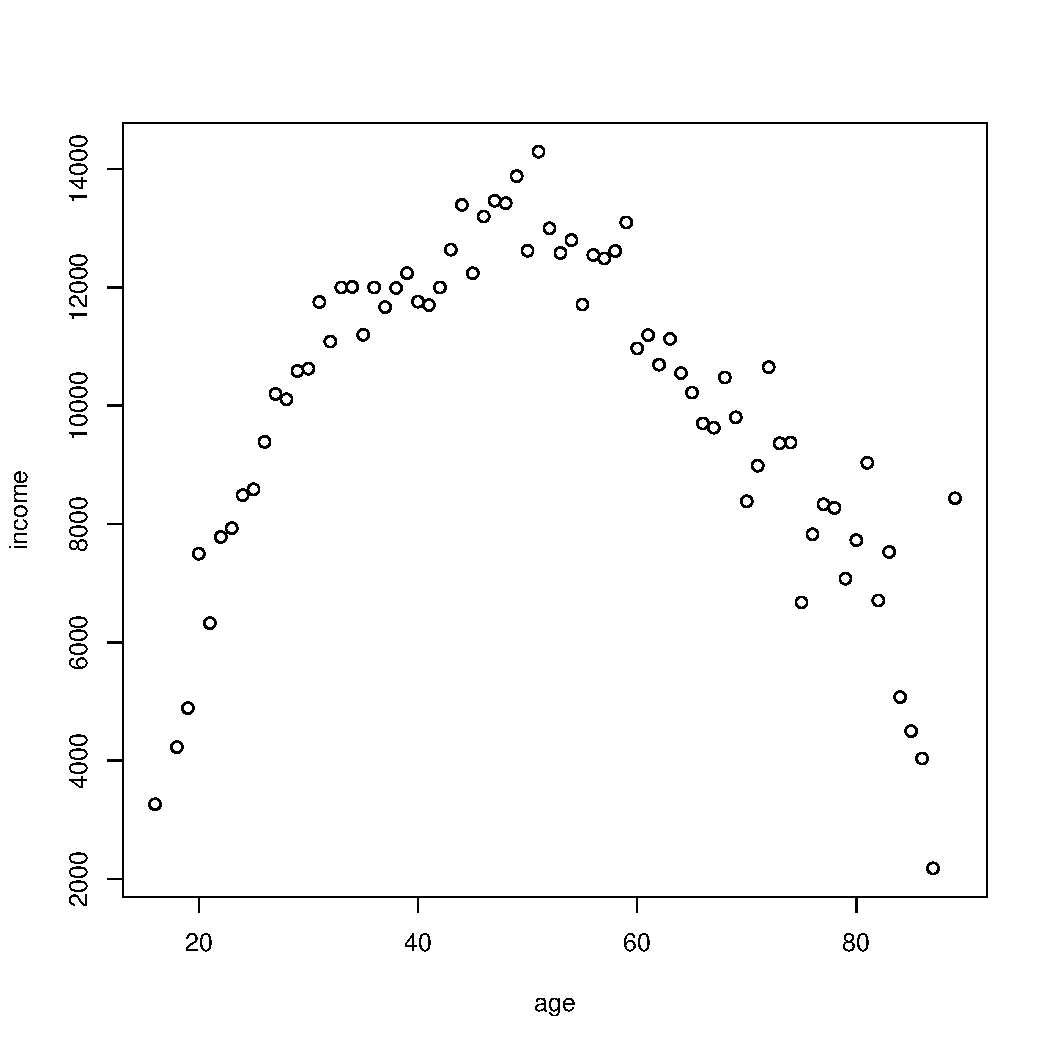
\includegraphics[scale=0.4]{figs/wage2median.pdf}
	\caption{Median Turkish salaries by age}
	\label{fig:tuik}
\end{figure}

\section{Default parameters}
Similarly to \citet{munk}, we start our simulation with a 25-year-old individual who invests in his/her retirement for 40 years until he/she reaches retirement at 65. Similarly to \citet{torul}, we set the default relative risk aversion coefficient for Turkish households at $1.5$, and the subjective discount rate --- at $0.89$.

\paragraph{}We deflate the nominal wages, stock and house prices by CPI and work with real variables.

\paragraph{}We obtain annual rate of return on stocks $6.69\%$ with volatility $38.44\%$, by annualizing long-term ARMA(2,2) forecasts of monthly return and volatility, based on historical BIST 30 data, mentioned above (see Appendix \ref{paramcalibx}).

\paragraph{}Similarly, we use long-term ARMA(1,1) forecast of monthly return and volatilities on housing, and find annual real rate of return on housing $0.67\%$ with $5.42\%$ volatility (see Appendix \ref{paramcaliby}).

\paragraph{}Risk-free rate $12\%$ is given by \citet{oecd} forecast\footnote{Data was obtained before the Turkish currency and debt crisis of 2018}, and, upon subtracting the medium-term inflation rate forecast $\pi = 9\%$ by \citet{tcmb}, is equal to $3\%$ per annum with zero volatility.

\paragraph{}We consider real wage growth rates separately for different types of agents, but before introducing heterogeneity, the ARMA(5,2) forecast gives the volatility $4\%$ (see Appendix \ref{paramcalibz}).

\paragraph{}In our simulation, the house-stock and house-wage contemporaneous correlations are given by $0.27$ and $0.35$ respectively. 

\paragraph{}Survival probabilities for all ages are provided by \citet{tuik2} and illustrated in Figure \ref{fig:surv}.

\begin{figure}[h!]
	\centering
	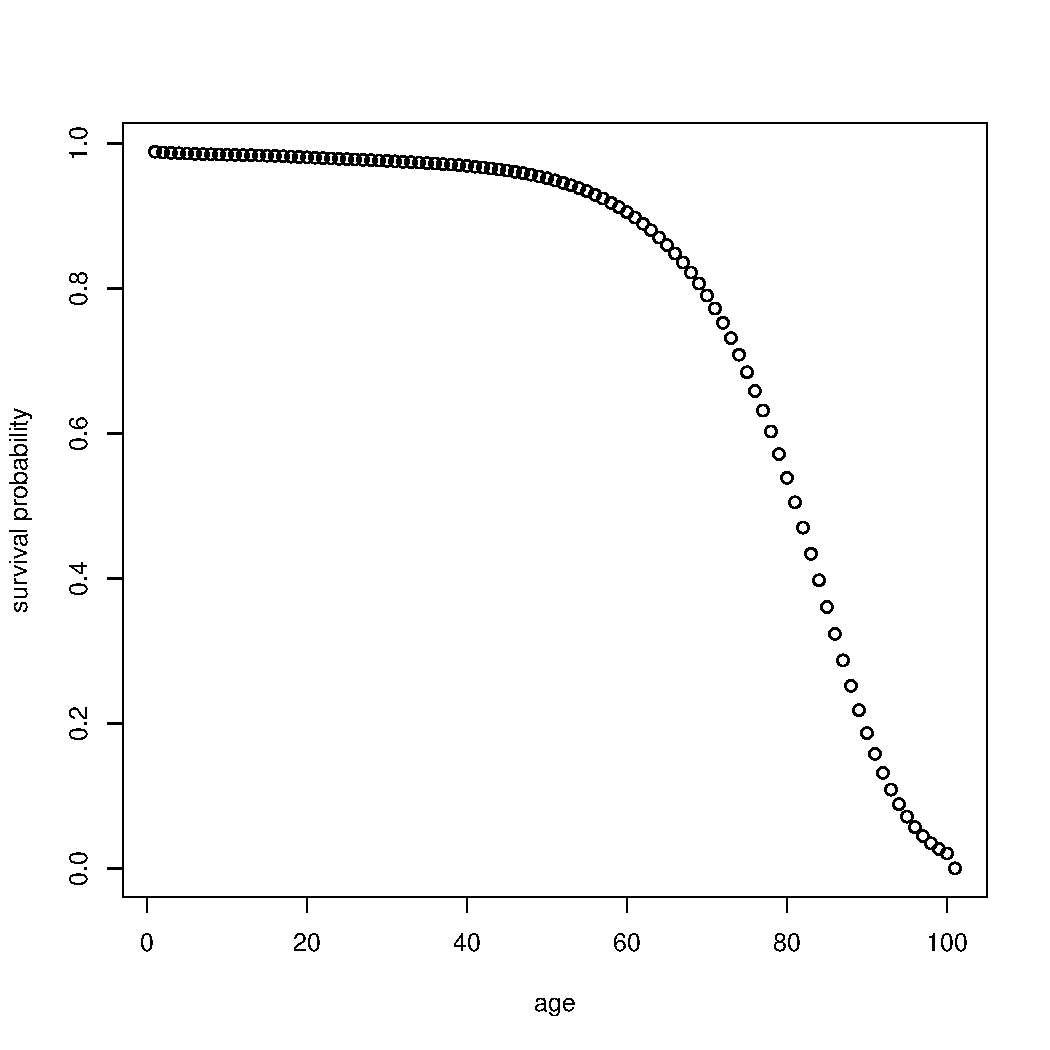
\includegraphics[scale=0.3]{figs/survival.pdf}
	\caption{Survival probabilities by age}
	\label{fig:surv}
\end{figure}

All of the above findings are summarized in Table \ref{table:default}. 

\begin{table}[h!]
	\centering
	\caption{Benchmark Parameters}
	\label{table:default}
	\begin{tabular}[c]{lll}
		\hline
		Parameter&Description&Value\\
		\hline
		$Y$&Beginning age&$25$\\
		$R$&Retirement age&$65$\\
		$T$&Lifespan (years)&$100$\\
		$\gamma$&Risk aversion&$1.5$\\
		$\beta$&Discount rate&$0.89$\\
		$r_f$&Risk-free rate&$0.03$\\
		\hline
		$\mu_s$&Expected stock returns&$0.0669$\\
		$\mu_h$&Expected housing returns&$0.0067$\\
		$\sigma_s$&Stock returns volatility&$0.3844$\\
		$\sigma_h$&Housing returns volatility&$0.0542$\\
		$\sigma_w$&Wage growth volatility&$0.036$\\
		$\rho_{hs}$&House-stock correlation&$0.24$\\
		$\rho_{hw}$&House-wage correlation&$0.37$\\
		\hline
		$p_{25}$&Survival probability at age 25&$0.978$\\
		$p_{65}$&Survival probability at age 65&$0.86$\\
		$p_{100}$&Survival probability at age 100&$0$\\	
		\hline
	\end{tabular}
\end{table}


\section{Heterogeneity parameters}
Combining the approaches of \citet{olear} and \citet{munk}, we use wage growth rate, stock-income correlation and relative risk aversion level, to model heterogeneities among agents.

\subsection{Heterogeneity in education}
We model the heterogeneity in education using differences in wage growth rates. Figure \ref{fig:wageeduc} shows the lifetime labor income series for different levels of education. Notice that the curves are almost flat for the lower education levels and hump-shaped for the higher.

\begin{figure}[h]
	\centering
	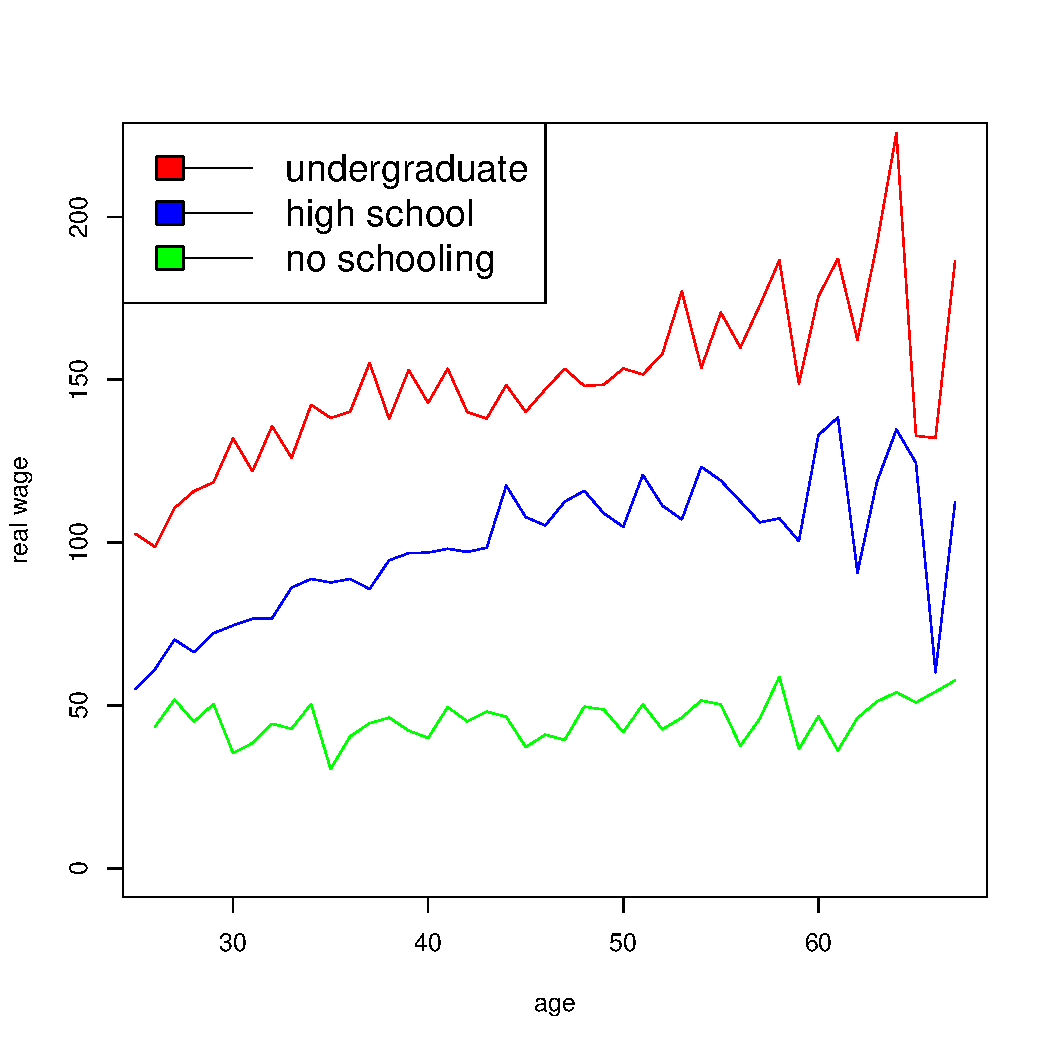
\includegraphics[scale=0.4]{figs/wage2educ.pdf}
	\caption{Lifetime real wage dynamics by education level.}
	\label{fig:wageeduc}
\end{figure}

We use undergraduate education, high school education, and no schooling, to model ``steep'', ``moderate'', and ``flat'' wage dynamics respectively. Performing regressions of wages on age, with kinks at $t=40$ and $t=55$:

\begin{equation}
	\Delta \log (wage_{it}) = \alpha_0 + \alpha_1 \cdot d_{40} + \alpha_2 \cdot d_{55}
\end{equation}

we estimate growth rates for different education levels, as summarized in Table \ref{table:dincome} (see Appendix \ref{paramcalibt} for regression results and line fits). 

\begin{table}[h!]
	\centering
	\caption{Estimated Benchmark Wage Growth Rates $\mu_w$}
	\label{table:dincome}
	\begin{tabular}[c]{l|ccc}
		Age&Flat&Moderate&Steep\\
		\hline
		25-40&0\%&3.8\%&2.2\%\\
		41-55&0\%&1.4\%&1.2\%\\
		56-65&0\%&0\%&1.5\%\\
	\end{tabular}
\end{table}

We assume steep wage earners (college graduates) to have a starting real salary of $100$, and moderate and flat wage earners to have a starting real salary of $50$. This is consistent with the historical data (see Figure \ref{fig:wageeduc}) and the relevant discussion by \citet{olear}. This difference in starting values also explains why ``steep'' wage growth rates are less than ``moderate'' ones.  

\subsection{Heterogeneity in sectors of work}

We model the heterogeneity work sectors using corresponding stock-wage correlations ($\rho_{ws}$). Figure \ref{fig:wagesec} illustrates how, during 2008 crisis, income in financial sectors ($\rho_{ws} = 0.44$) dropped drastically, while it was unaffected in education and agriculture ($\rho_{ws} = 0.08$).
\begin{figure}[h!]
	\centering
	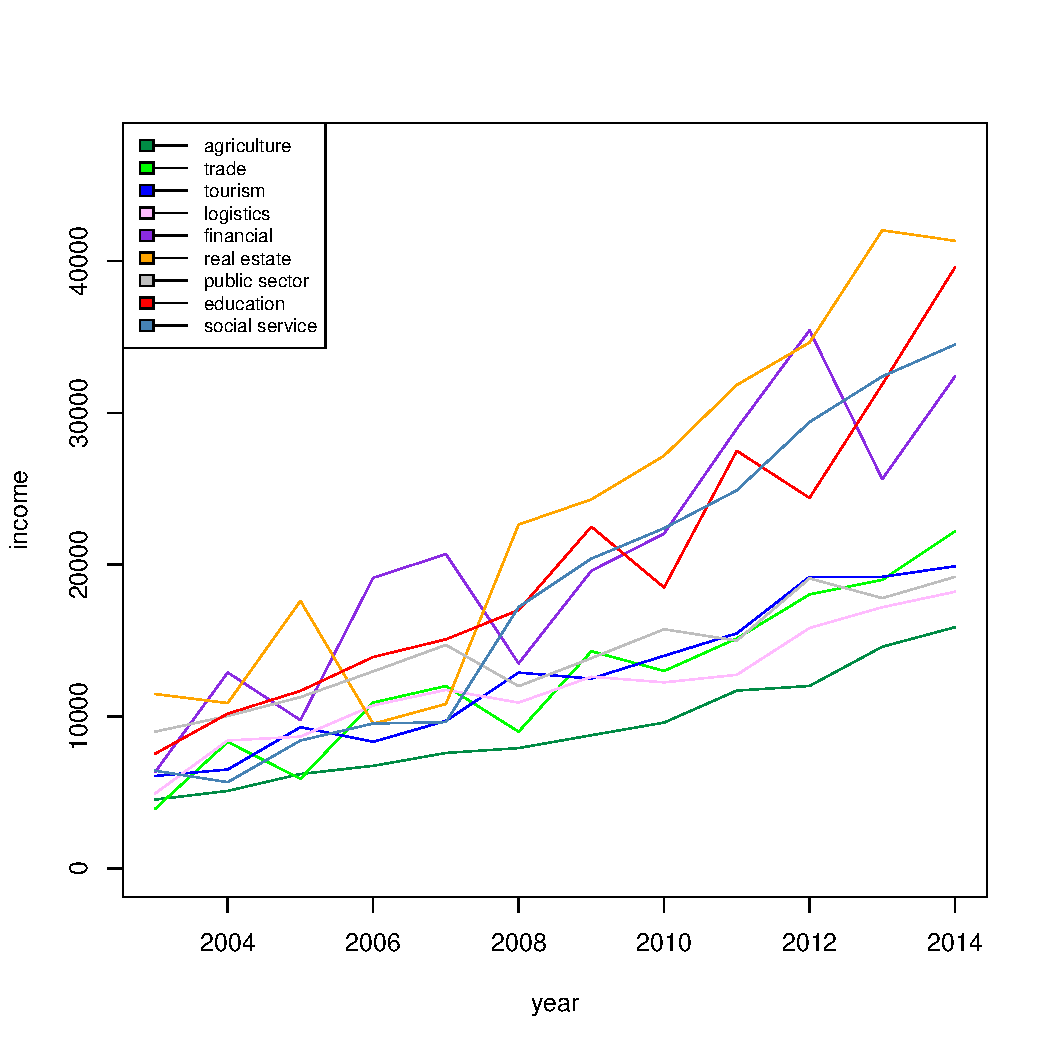
\includegraphics[scale=0.4]{figs/wage2sec.pdf}
	\caption{Historical real wage dynamics by sector.}
	\label{fig:wagesec}
\end{figure}

We use three measures of $\rho_{sw}$ for our benchmark: $0$, $0.2$ and $0.4$ (see Table \ref{table:wagesec}).


\begin{table}[h!]
	\centering
	\caption{Benchmark Wage to Stock Correlations}
	\label{table:wagesec}
	\begin{tabular}[c]{c|ccc}
		&Low&Moderate&High\\
		\hline
		$\rho_{sw}$&0&0.2&0.4
	\end{tabular}
\end{table}


\subsection{Individual heterogeneity}

We model individual heterogeneity using different risk aversion levels of investors, as summarized in Table \ref{table:riskave}.

\begin{table}[h!]
	\centering
	\caption{Coefficients of Risk Aversion}
	\label{table:riskave}
	\begin{tabular}[c]{r|cccc}
		Values&default&low&moderate&high\\
		\hline
		$\gamma$&1.5&3&5&10\\
	\end{tabular}
\end{table}

\section{Capital series}

\subsection{Human capital}
Human capital at any period is the discounted sum of all future wages until retirement with the discount factor $r_f$. To construct the individualized capital we used steep, moderate and flat wage series mentioned in the previous section. Figure \ref{fig:humcap} illustrates the current human capital for flat, moderate, and steep wages for every age. 

\subsection{Financial capital}

Financial capital evolves according to dynamic investment diagram in Figure \ref{fig:invdiag}. Every period, a certain percentage $c$ ($3\%$ for Turkey) of the wage $w_t$ is invested in a retirement portfolio, while the previously invested amount accrues interest at portfolio rate of return. Figure \ref{fig:fincap} demonstrates the evolution of financial capital and its confidence interval for a naive fixed investment strategy ($50\%$ in stocks and $50\%$ in bonds) by an individual with ``steep'' wage curve.

\begin{figure}[h!]
	\centering
    \begin{minipage}{0.45\textwidth}
		\centering
		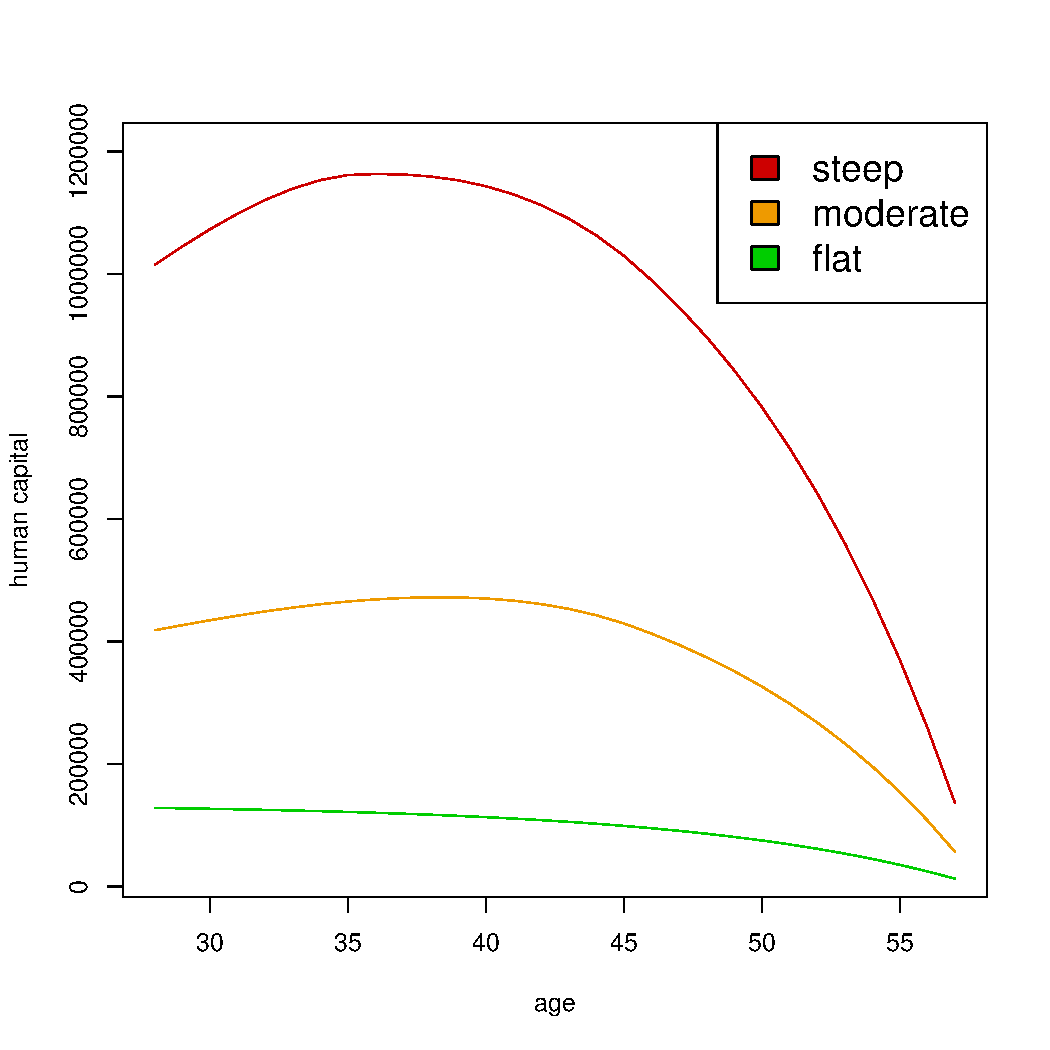
\includegraphics[scale=0.4]{figs/humancapital.pdf}
		\caption{Human capital at every age for steep, moderate and flat wages.}
		\label{fig:humcap}
	\end{minipage}
	\hfill
    \begin{minipage}{0.45\textwidth}
		\centering
		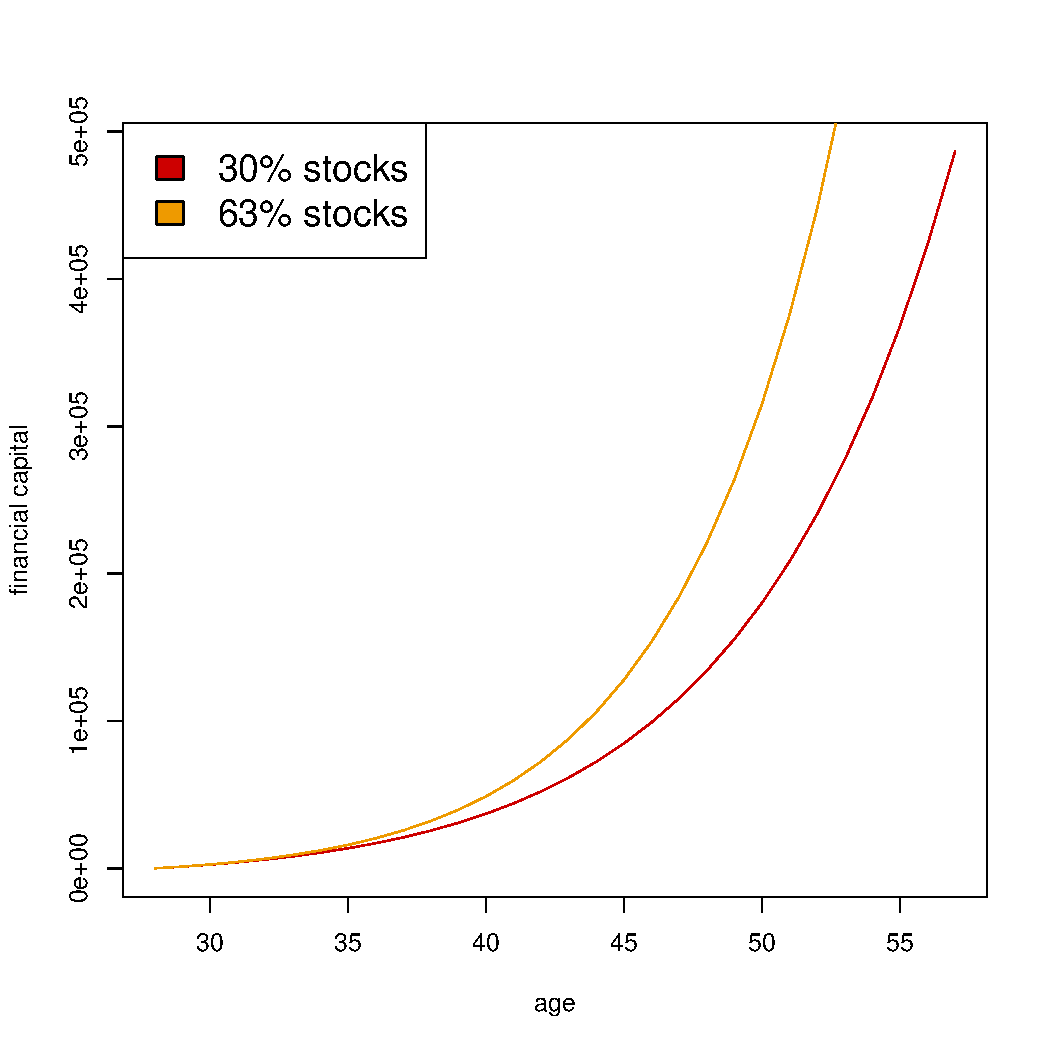
\includegraphics[scale=0.4]{figs/fincapital.pdf}
		\caption{Financial capital at every age.}
		\label{fig:fincap}
	\end{minipage}
\end{figure}

\begin{figure}[h!]
	\centering
	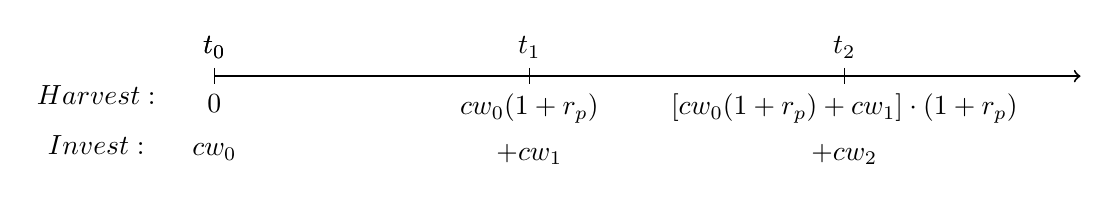
\begin{tikzpicture}
		\draw [->, line width=0.25mm] (0,0) -- (11,0);
		\foreach \x in {0,4,8}
			\draw (\x cm,3pt) -- (\x cm, -3pt);
		\draw (0,0) node[below=21pt] {$ cw_0 $} node[above=3pt] {$ t_0 $};
    	\draw (4,0) node[below=21pt] {$ +cw_1 $} node[above=3pt] {$ t_1 $};
    	\draw (8,0) node[below=21pt] {$ +cw_2 $} node[above=3pt] {$ t_2 $};
		\draw (0,0) node[below=3pt] {$ 0 $} node[above=3pt] {$ t_0 $};
    	\draw (4,0) node[below=3pt] {$ cw_0(1+r_p) $};
    	\draw (8,0) node[below=3pt] {$ \left[cw_0(1+r_p) + cw_1 \right] \cdot (1+r_p) $};
	    \draw (-1.5,0) node[below=18pt] {$ Invest: $};
    	\draw (-1.5,0) node[below=0pt] {$ Harvest: $};
	\end{tikzpicture}
	\caption{Law of motion of financial capital.}
	\label{fig:invdiag}
\end{figure}


\section{Investment strategies}

Below, we present the life-cycle investment strategies to be benchmarked.

\subsection{Homogeneous life-cycles}

Homogeneous life-cycles are strategies, common to all individuals, regardless of their idiosyncratic characteristics. We benchmark strategies given by equations \ref{eq:markowitz}, \ref{eq:stominus}, \ref{eq:cgm}, and an aggressive portfolio allocation, offered by Turkish banks ($60\%$ in stocks, $40\%$ in bonds). Figure \ref{fig:defaults} illustrates the stock shares in these investment strategies.


\begin{figure}[h!]
	\centering
	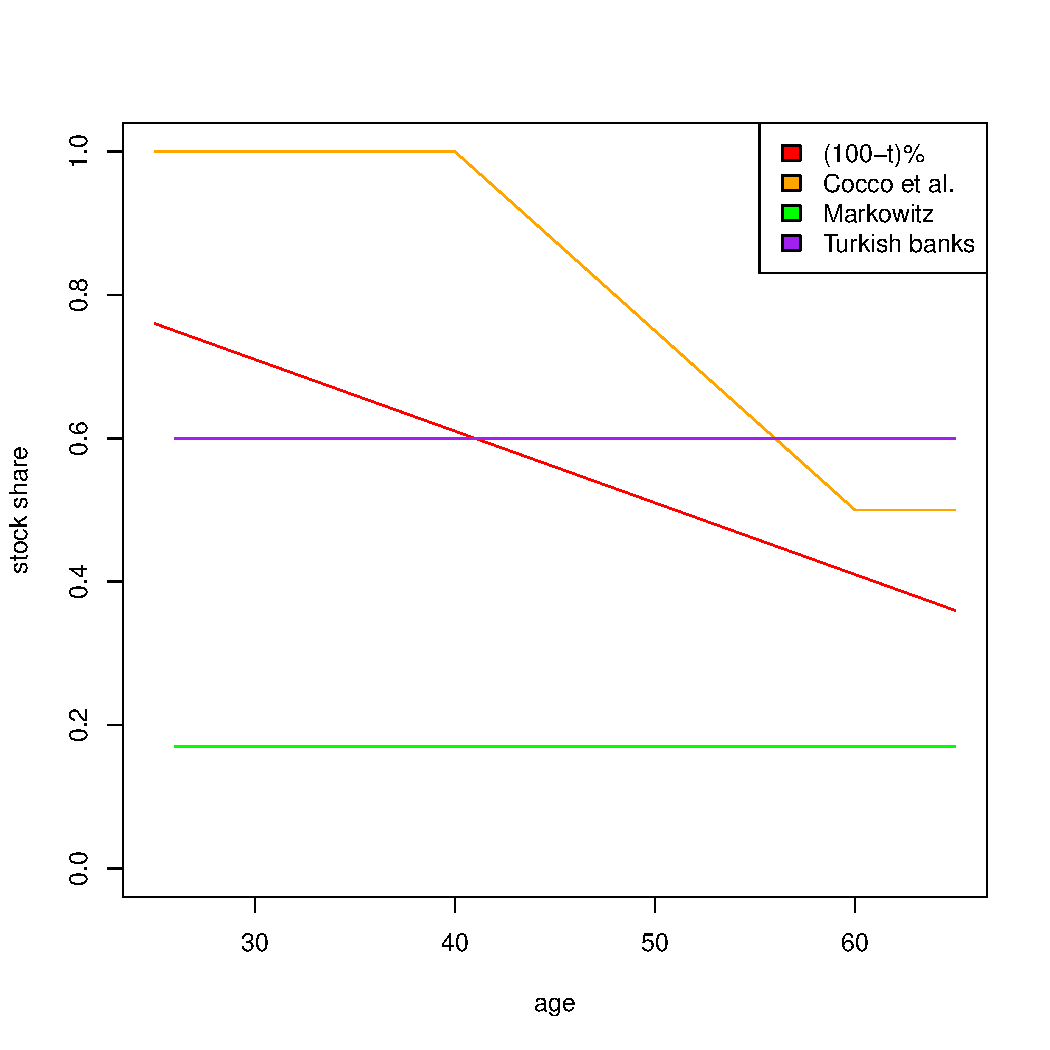
\includegraphics[scale=0.4]{figs/defaults.pdf}
	\caption{Share of stocks in a portfolio at every age, proposed by homogeneous life-cycle strategies}
	\label{fig:defaults}
\end{figure}


\subsection{Heterogeneous life-cycles}

Heterogeneous life-cycles take idiosyncratic characteristics into consideration. We benchmark strategies by \citet{bodie} (see Equation \ref{eq:bodie}), and \citet{munk} (see Equation \ref{eq:munkno}), which are illustrated in Figure \ref{fig:individs} by blue and red curves respectively. The dashed lines illustrate the $68\%$-confidence interval ($\pm 1\sigma$). The figure proposes younger investors to allocate all of their funds in stocks, and gradually, through life, decrease their share in the portfolio --- the more risk-averse they are or the flatter their wage curve is, the sooner. It also shows that, other things being equal, \citet{munk}'s strategy without housing, is less aggressive than \citet{bodie}'s, which is consistent with equations \ref{eq:bodie} and \ref{eq:munkno}. 

\begin{figure}[h!]
	\centering
    \begin{subfigure}{0.45\textwidth}
		\centering
		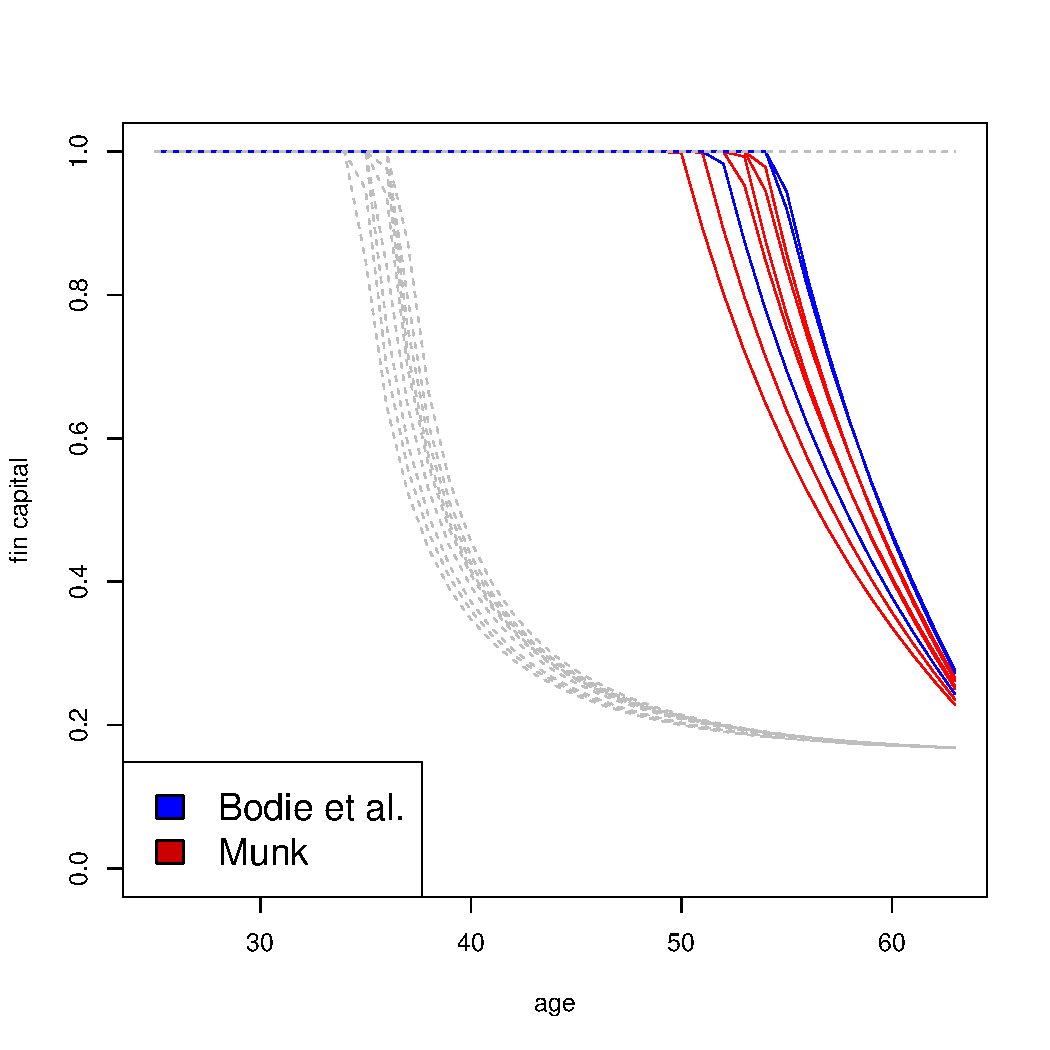
\includegraphics[scale=0.3]{figs/individuals15.pdf}
		\caption{$\gamma = 1.5$}
	\end{subfigure}
	\hfill
    \begin{subfigure}{0.45\textwidth}
		\centering
		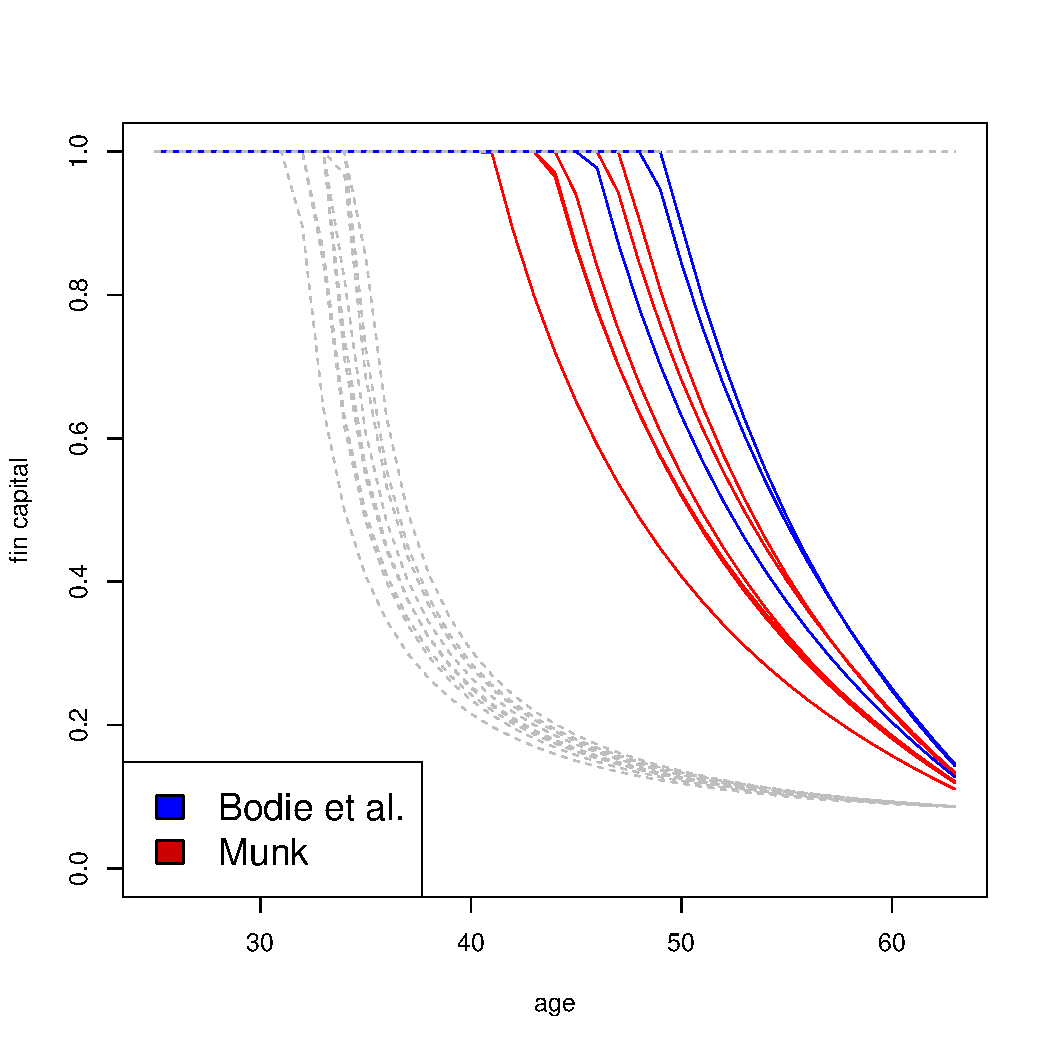
\includegraphics[scale=0.3]{figs/individuals3.pdf}
		\caption{$\gamma = 3$}
	\end{subfigure}
\end{figure}
\begin{figure}[H]\ContinuedFloat
    \begin{subfigure}{0.45\textwidth}
		\centering
		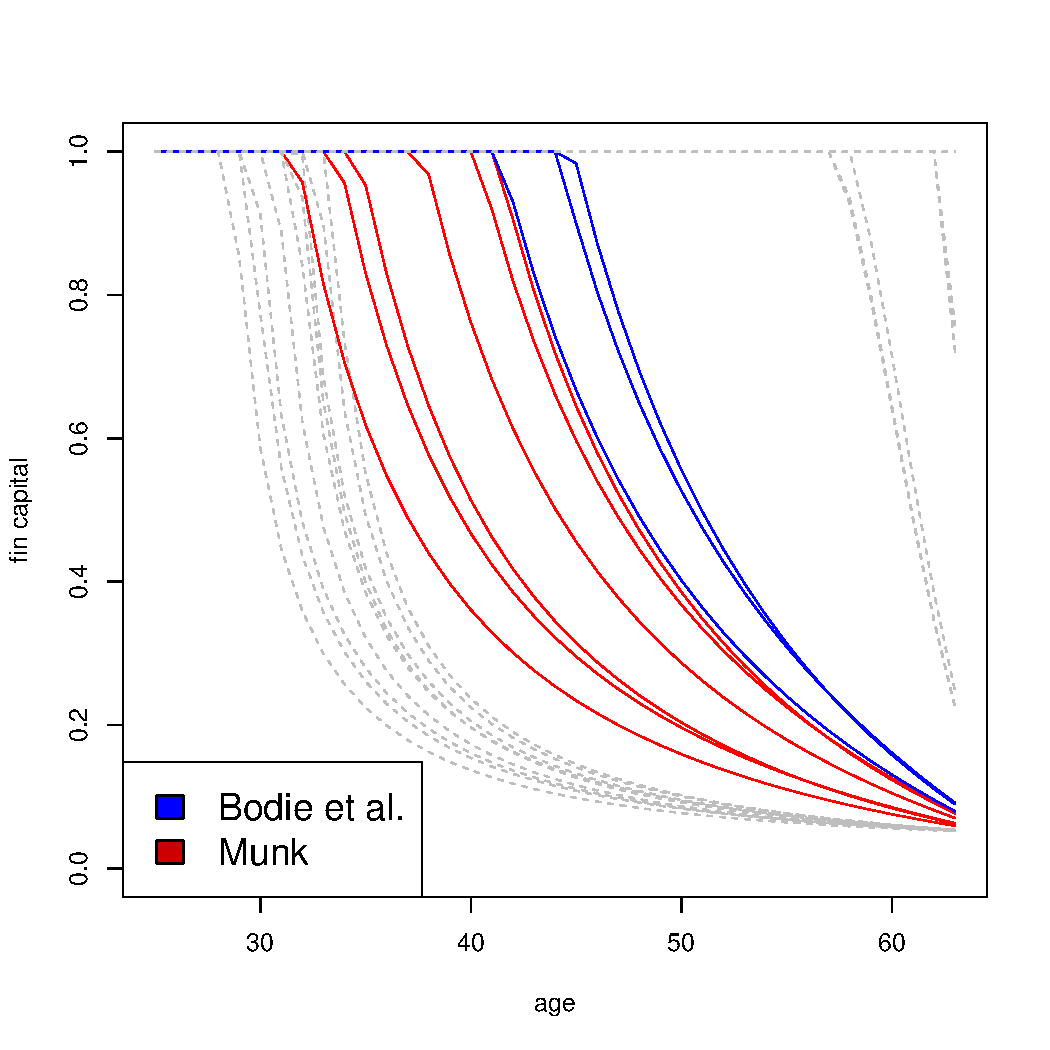
\includegraphics[scale=0.3]{figs/individuals5.pdf}
		\caption{$\gamma = 5$}
	\end{subfigure}
	\hfill
    \begin{subfigure}{0.45\textwidth}
		\centering
		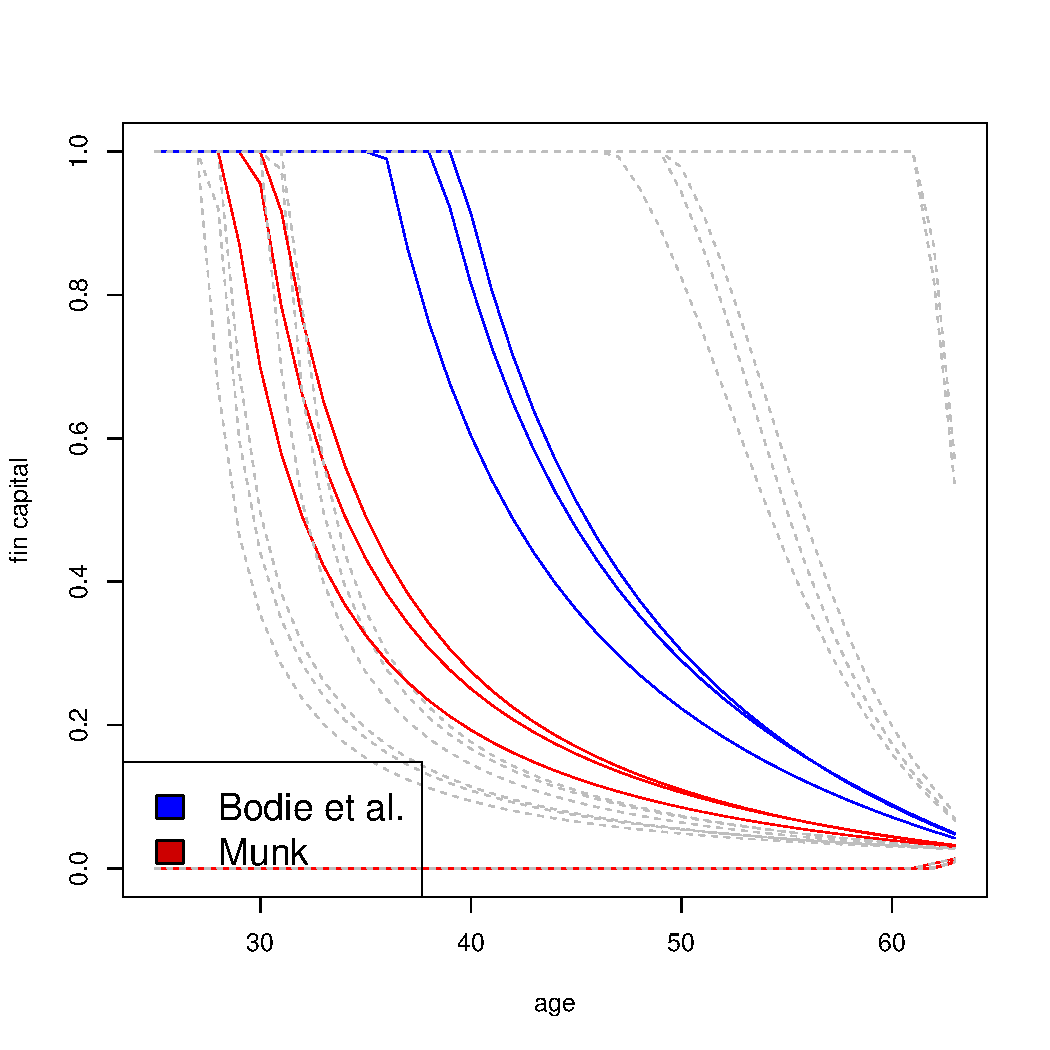
\includegraphics[scale=0.3]{figs/individuals10.pdf}
		\caption{$\gamma = 10$}
	\end{subfigure}
	\caption{Shares of stocks in a portfolio, suggested by \citet{bodie} and \citet{munk}.}
	\label{fig:individs}
\end{figure}


Figure \ref{fig:munkh} shows the stock and house shares, suggested by \citet{munk} for flat, moderate and steep labor income curves, low, moderate and high stock-wage correlations, and different levels of risk aversion. It confirms that steeper labor income curves results in a larger share of stocks in portfolio, and the more risk averse individuals are, the sooner they decrease both housing and stock investment, and buy more bonds.

\clearpage
\begin{figure}[H]
	\centering
    \begin{subfigure}{0.45\textwidth}
		\centering
		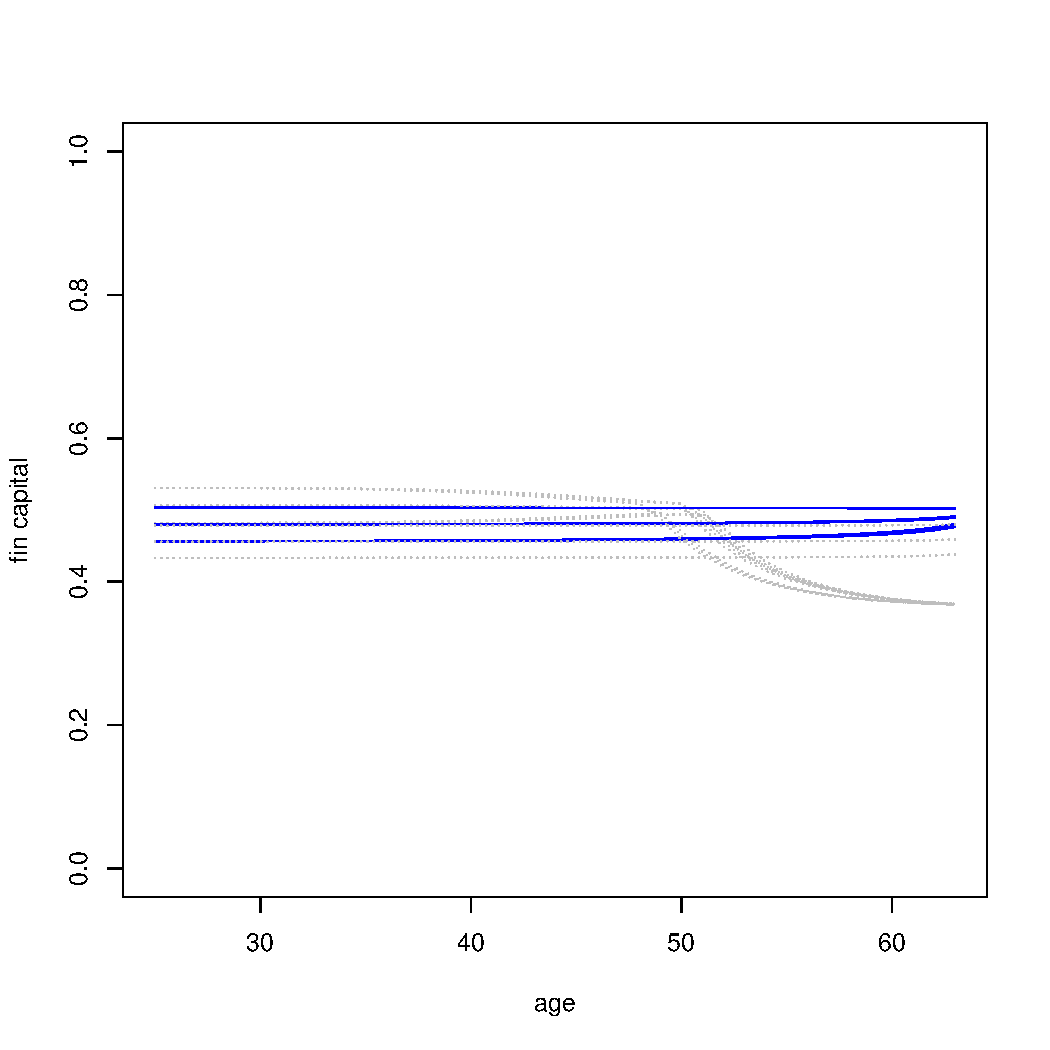
\includegraphics[scale=0.25]{figs/smunkhouse15.pdf}
		\caption{Stocks for $\gamma = 1.5$}
	\end{subfigure}
	\hfill
    \begin{subfigure}{0.45\textwidth}
		\centering
		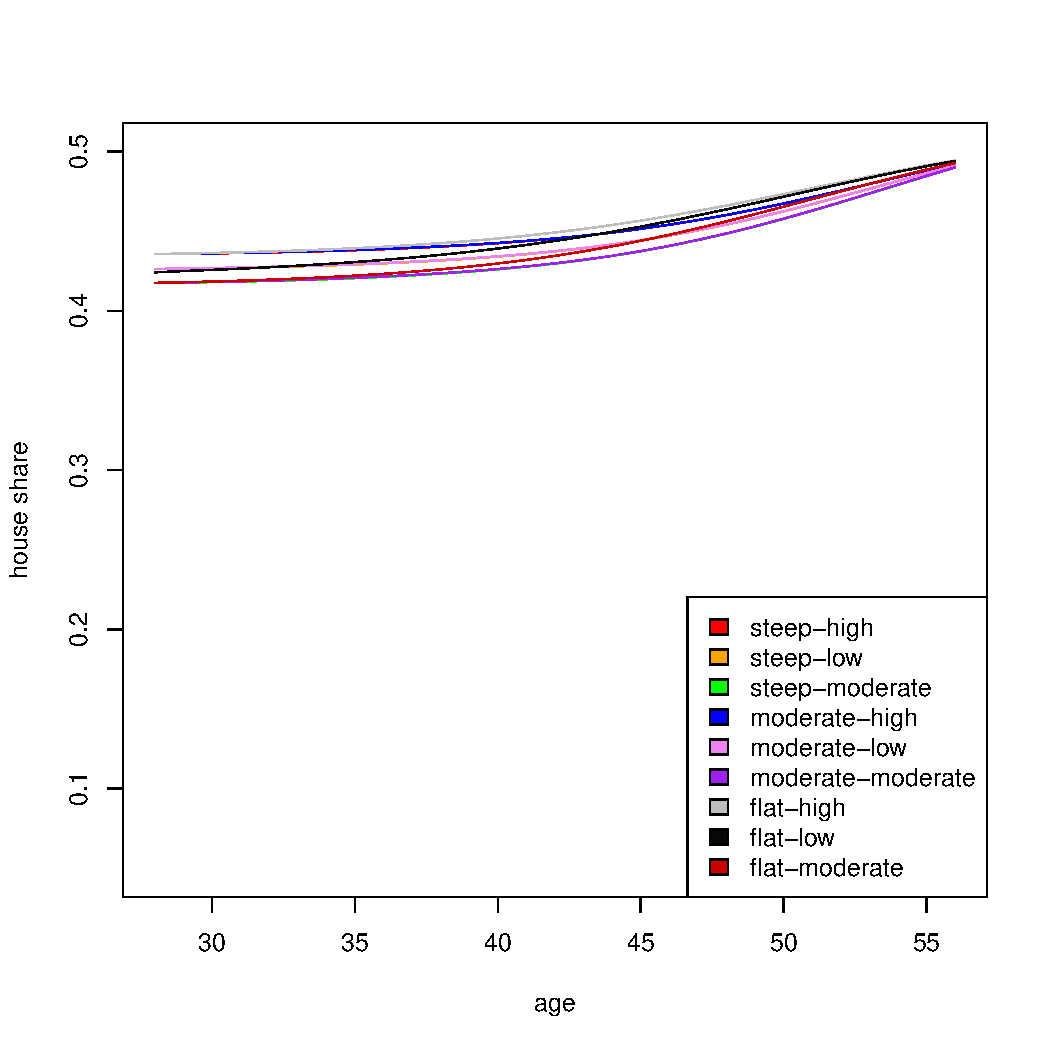
\includegraphics[scale=0.25]{figs/hmunkhouse15.pdf}
		\caption{Housing for $\gamma = 1.5$}
	\end{subfigure}
\end{figure}
\begin{figure}[H]\ContinuedFloat
    \begin{subfigure}{0.45\textwidth}
		\centering
		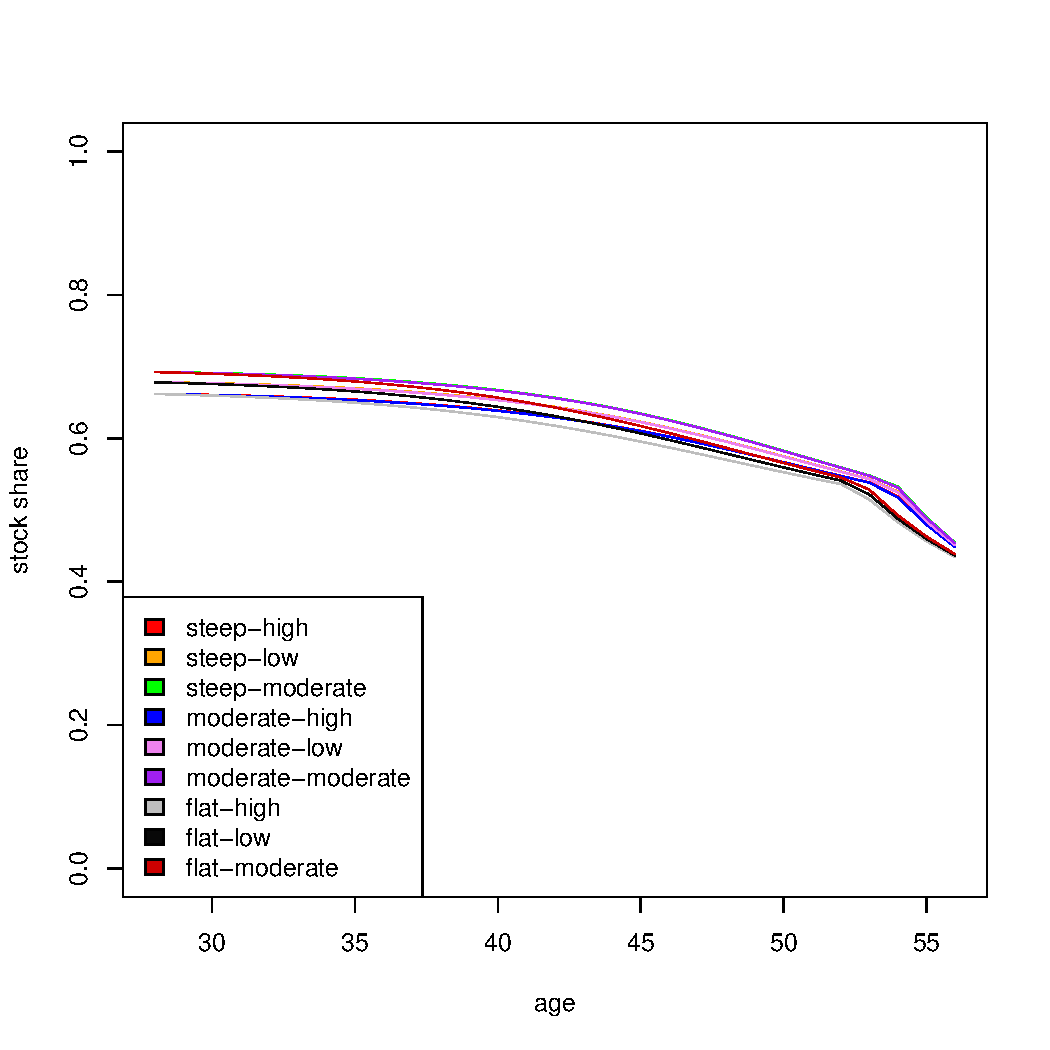
\includegraphics[scale=0.25]{figs/smunkhouse3.pdf}
		\caption{Stocks for $\gamma = 3$}
	\end{subfigure}
	\hfill
    \begin{subfigure}{0.45\textwidth}
		\centering
		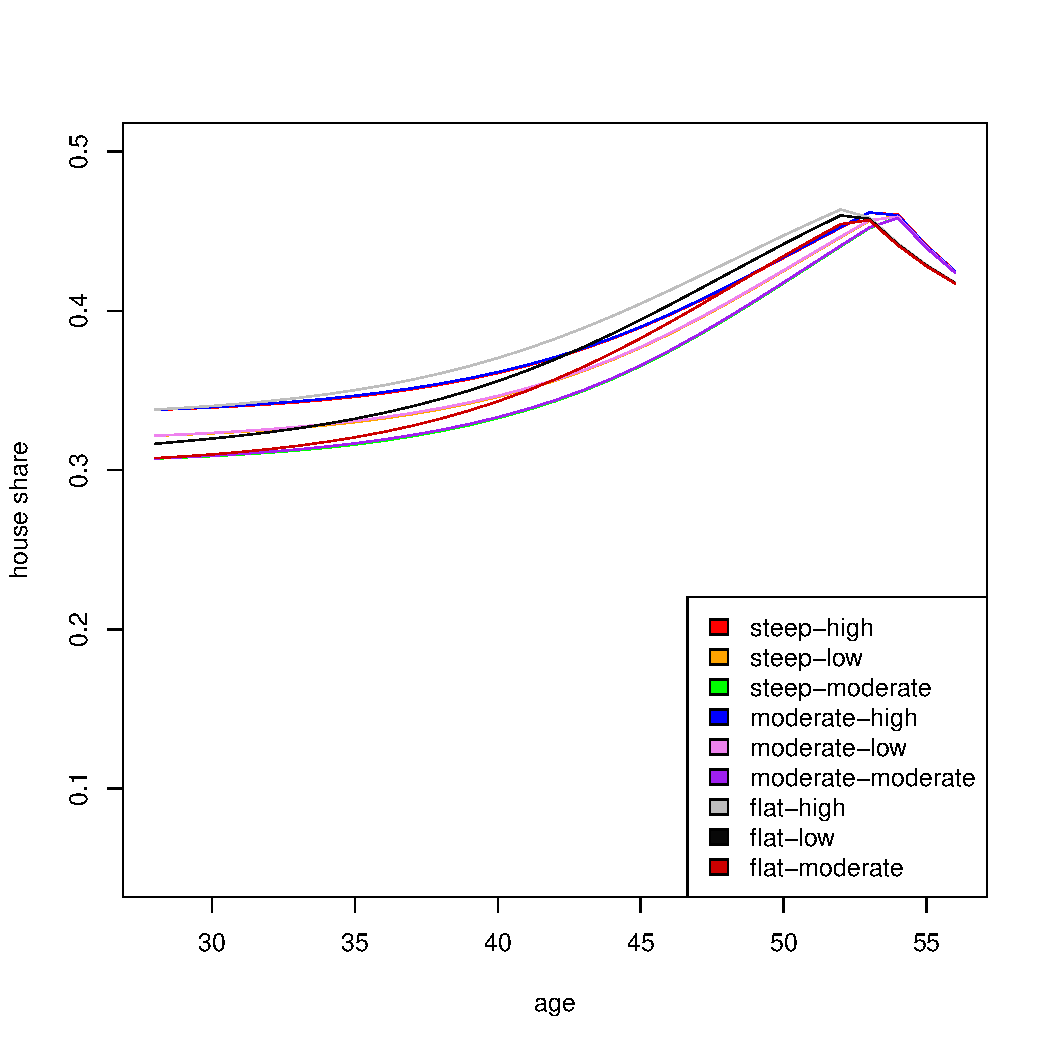
\includegraphics[scale=0.25]{figs/hmunkhouse3.pdf}
		\caption{Housing for $\gamma = 3$}
	\end{subfigure}
\end{figure}
\begin{figure}[H]\ContinuedFloat
    \begin{subfigure}{0.45\textwidth}
		\centering
		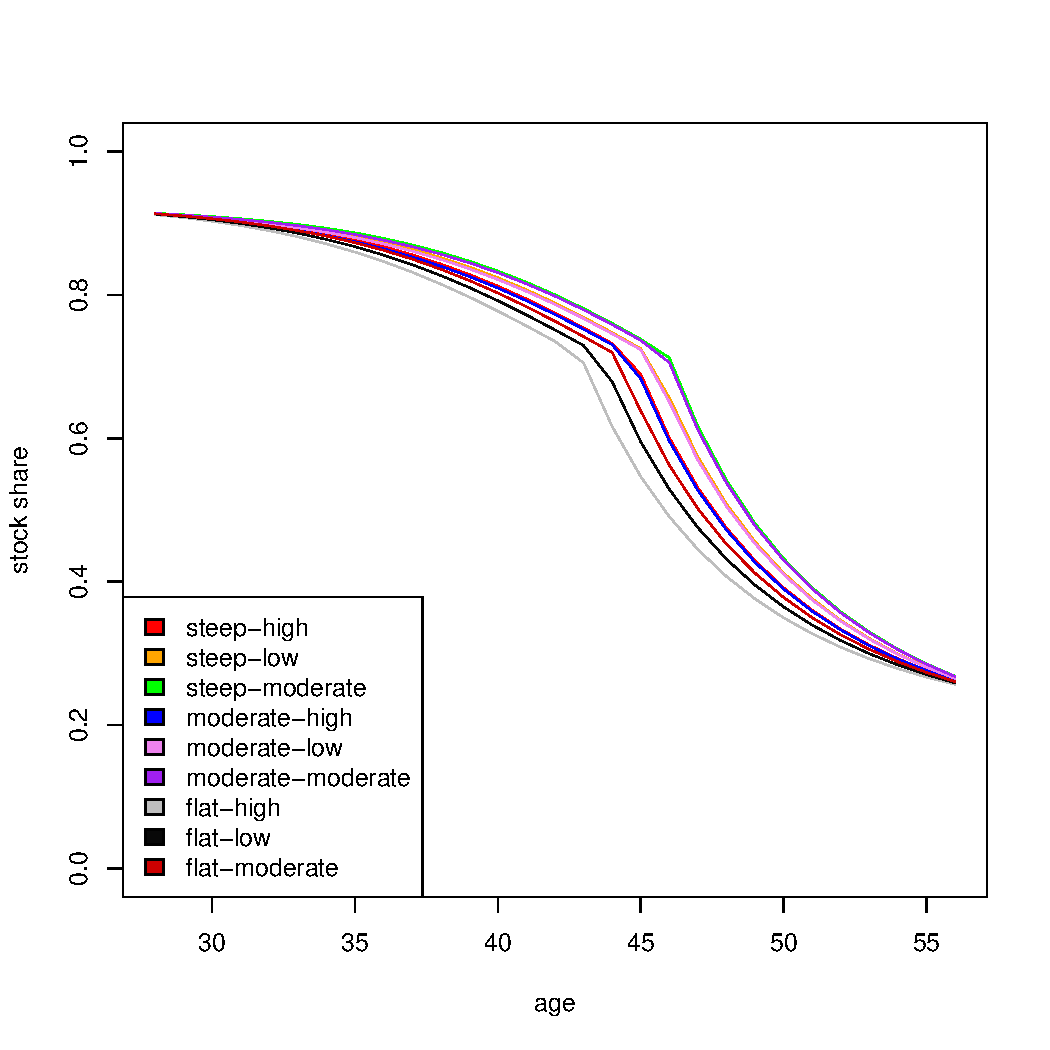
\includegraphics[scale=0.25]{figs/smunkhouse5.pdf}
		\caption{Stocks for $\gamma = 5$}
	\end{subfigure}
	\hfill
    \begin{subfigure}{0.45\textwidth}
		\centering
		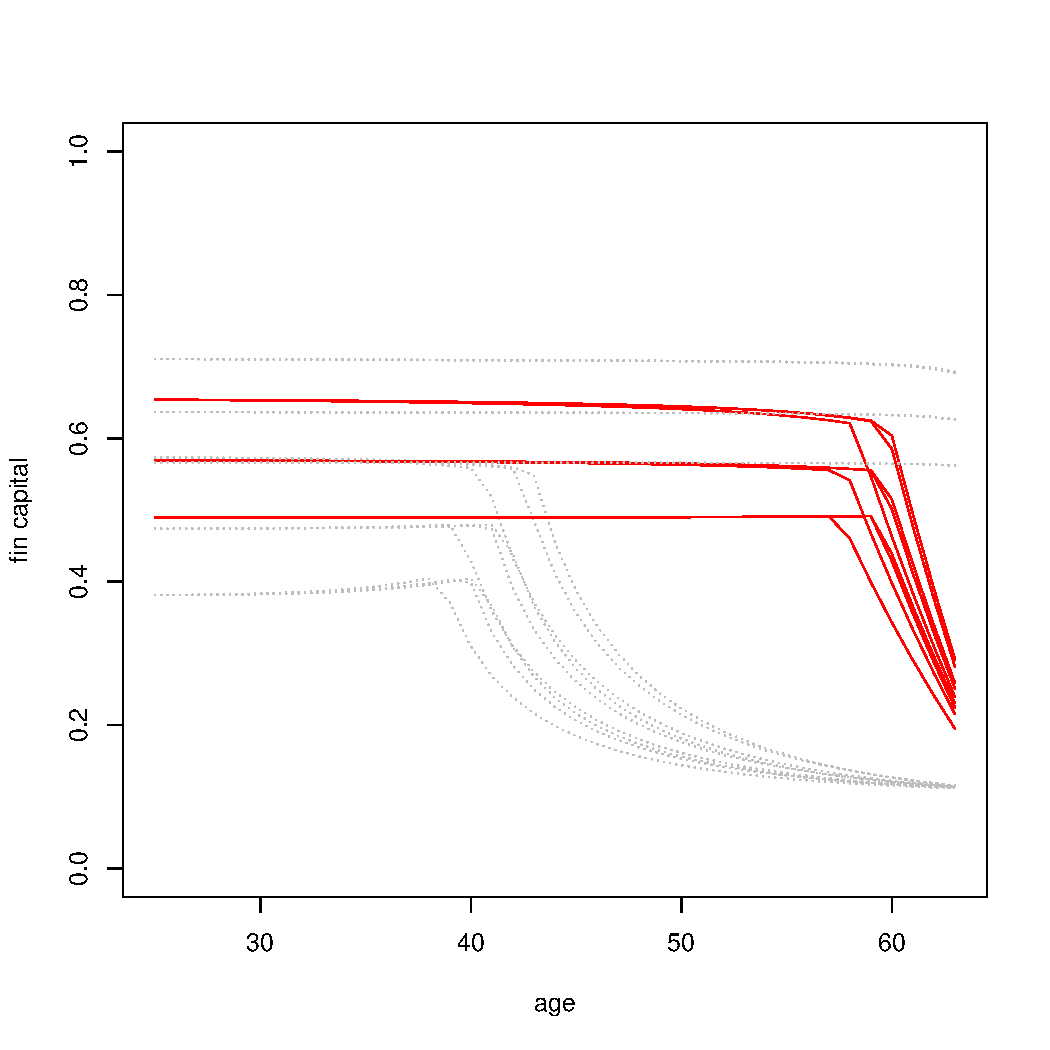
\includegraphics[scale=0.25]{figs/hmunkhouse5.pdf}
		\caption{Housing for $\gamma = 5$}
	\end{subfigure}
\end{figure}
\begin{figure}[H]\ContinuedFloat
    \begin{subfigure}{0.45\textwidth}
		\centering
		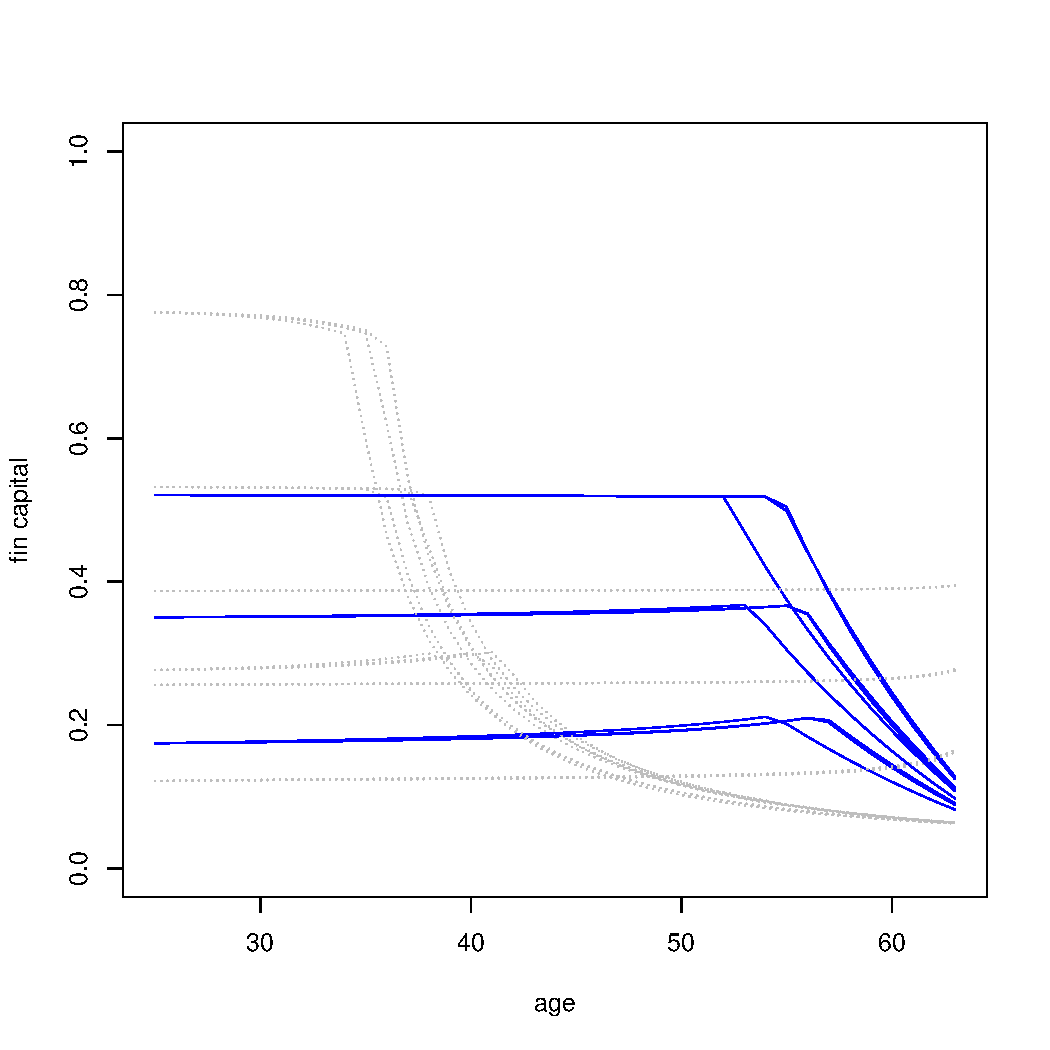
\includegraphics[scale=0.25]{figs/smunkhouse10.pdf}
		\caption{Stocks for $\gamma = 10$}
	\end{subfigure}
	\hfill
    \begin{subfigure}{0.45\textwidth}
		\centering
		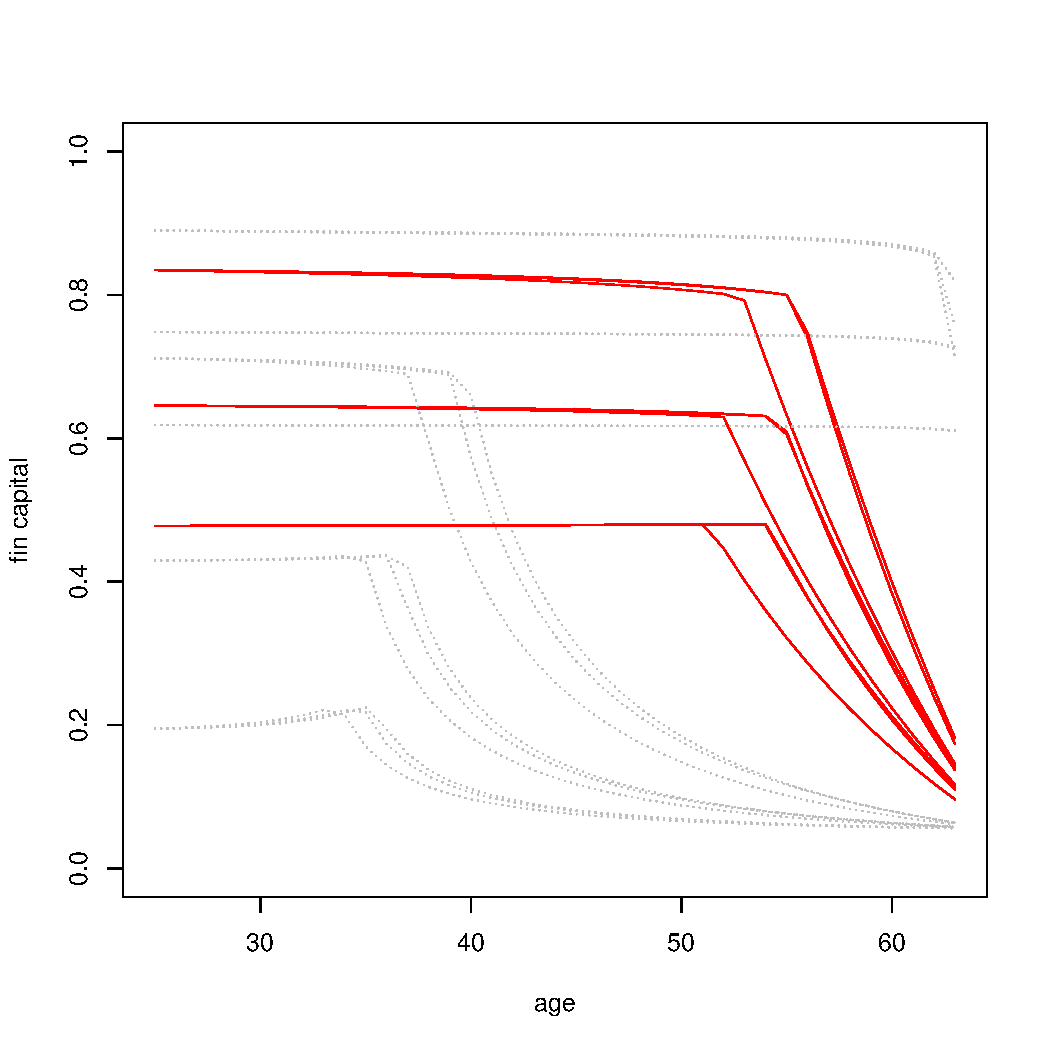
\includegraphics[scale=0.25]{figs/hmunkhouse10.pdf}
		\caption{Housing for $\gamma = 10$}
	\end{subfigure}
	\caption{Munk's stock and housing shares for different wage growth, stock-wage correlation and risk aversion levels}
	\label{fig:munkh}
\end{figure}
